% 附录 AC：等离子体数值方法——从 PIC 到 MHD（v1.26.7 新增）
% 数值唯一来源：tools/calc/appAC_calc.py -> tools/calc/appAC_calc.txt（正文与门禁 P35 的唯一来源）
% 单位写法：m / s / rad s^-1 / Hz / V m^-1 / K / Pa / kg m^-3，全部走 \mathrm{}，不放中文字符进数学字体。
% 版权口径：只借鉴经典教材与文献的物理结论、公式形式与题型；文字、数值与表格自拟并独立复算。
% 离线环境无法核验 DOI，故只给书名、作者、年份、卷期页。
% 分工：M--AB 讲的是物理（加热、边界、约束、破裂、快粒子、辐射、强场、堆工程、替代位形、空间天体）；
%       附录 G 是软件上手教程，附录 I 讲学习策略，附录 Q 讲诊断误差；
%       本附录补最后一环：同一批方程，怎么变成可信的计算。
% 引用的全部数字由 tools/calc/appAC_calc.py 现算；脚本内声明的输入见 AC.1 开头的表。

\section{分辨率：先算三个长度与三个时间}
\label{sec:app-ac-resolve}
\setlength{\emergencystretch}{3em}

前面二十几个附录都在算「物理量等于多少」。本附录换一个问题：\textbf{这些量该怎么算出来}。
数值模拟的第一件事不是挑算法，而是回答「要分辨什么」——分辨不了的东西，
再好的格式也只是把误差放大得更整齐。

取与附录 M 到 AB 同一个工作点：$n_e=1.0\times10^{20}\ \mathrm{m^{-3}}$、
$T_e=9.194\ \mathrm{keV}$、$B=5.3\ \mathrm{T}$。第一件要分辨的事是德拜屏蔽：

\begin{equation}
\lambda_{De}=\sqrt{\frac{\epsilon_0 k_B T_e}{n_e e^2}}
=7.12806\times10^{-5}\ \mathrm{m}=71.28\ \mathrm{\mu m}.
\label{eq:app-ac-debye}
\end{equation}

这是 PIC 的\textbf{网格下限}：网格步长必须小于德拜长度。原因是网格只能「看见」比它粗的
电荷分离；一旦 $\Delta x>\lambda_{De}$，网格会把本该被屏蔽掉的静电场当成真实场留下来，
于是它自己长出一种纯数值的不稳定性——有限网格不稳定性，与物理毫无关系。

第三件事是时间。粒子有两个时标：绕磁力线转和随等离子体振荡。取工作点的两个频率：

\begin{equation}
\begin{aligned}
&\omega_{pe}=\sqrt{\frac{n_e e^2}{\epsilon_0 m_e}}=5.64146\times10^{11}\ \mathrm{rad\,s^{-1}}
=89.787\ \mathrm{GHz},\\
&\omega_{ce}=\frac{eB}{m_e}=9.32175\times10^{11}\ \mathrm{rad\,s^{-1}}
=148.36\ \mathrm{GHz}.
\end{aligned}
\label{eq:app-ac-freq}
\end{equation}

回旋频率比等离子体频率还高 $1.65236$ 倍，所以在强磁场装置里，
\textbf{限制步长的不是等离子体振荡，而是回旋运动}。取「每步转过的角度不超过 $0.2$ 弧度」，
两条判据分别是 $0.2/\omega_{pe}=3.54518\times10^{-13}\ \mathrm{s}$ 与
$0.2/\omega_{ce}=2.14552\times10^{-13}\ \mathrm{s}$，后者更紧。
时间步长就定在后者，于是

\begin{equation}
\Delta t=0.2/\omega_{ce}=2.14552\times10^{-13}\ \mathrm{s},
\qquad
v_{the}\Delta t=8.62771\times10^{-6}\ \mathrm{m}=0.12104\ \lambda_{De},
\label{eq:app-ac-step}
\end{equation}

也就是每个时间步里电子只走约九分之一的德拜长度——网格与步长是配套选的，不能各管各。

第四个量不是判据，而是\textbf{信噪比}：德拜球里有多少个粒子。

\begin{equation}
N_D=n_e\lambda_{De}^3=3.62171\times10^{7}.
\label{eq:app-ac-nd}
\end{equation}

三千六百万个粒子在一个德拜球里，说明这个工作点的等离子体是\textbf{极其连续}的：
真实装置里几乎每个「点」都有海量粒子。这条数字会在 AC.4 变成一句很贵的结论——
我们只能用几千万个「超级粒子」代替它。

最后一条判据常被忽略：模拟窗口内要不要算碰撞？用 Spitzer 公式（库仑对数取 $17$，
写在脚本里作为声明输入）估算电子—离子碰撞时间：

\begin{equation}
\tau_{ei}=\frac{3(2\pi)^{3/2}\epsilon_0^2 m_e^2 v_{the}^3}{n_e e^4 Z_{\mathrm{eff}}\ln\Lambda}
=8.92144\times10^{-5}\ \mathrm{s},
\qquad
\frac{t_{\mathrm{sim}}}{\tau_{ei}}=1.9869\times10^{-5}.
\label{eq:app-ac-collision}
\end{equation}

模拟窗口只有 $1.77259\ \mathrm{ns}$，比碰撞时间长不到五万分之一。
所以\textbf{不加碰撞是物理判断，不是偷懒}：在这个窗口里，碰撞根本没来得及发生。

\begin{table}[htbp]
\centering
\small
\begin{tabular}{p{2.4cm}p{3.2cm}p{3.5cm}p{4.2cm}}
\toprule
要分辨的 & 判据 & 本工作点的数 & 不满足会怎样 \\
\midrule
德拜屏蔽 & $\Delta x\le\lambda_{De}$ & $\lambda_{De}=7.12806\times10^{-5}\ \mathrm{m}$ & 有限网格不稳定性 \\
等离子体振荡 & $\Delta t\le0.2/\omega_{pe}$ & $3.54518\times10^{-13}\ \mathrm{s}$ & 越步，能量凭空长 \\
电子回旋 & $\Delta t\le0.2/\omega_{ce}$ & $2.14552\times10^{-13}\ \mathrm{s}$ & 回旋轨道被算成多边形 \\
粒子离散噪声 & $N_p\gg1$（每格） & 取 $20$ & 噪声淹没信号（AC.4） \\
边界距离 & $L\gg\lambda_{De}$ & $L=100\lambda_{De}=0.71281\ \mathrm{cm}$ & 边界反射污染物理区 \\
碰撞 & $t_{\mathrm{sim}}\ll\tau_{ei}$ & $t_{\mathrm{sim}}/\tau_{ei}=1.9869\times10^{-5}$ & 需显式加碰撞模块 \\
\bottomrule
\end{tabular}
\caption{PIC 模拟开工前必须回答的六个问题。前三行是硬判据，后三行是设计选择。}
\label{tab:app-ac-resolution}
\end{table}

\begin{tip}{先算分辨率，再谈算法}{tip-app-ac-resolve}
几乎所有「模拟跑出来不对」的案例，第一现场都不在算法，而在分辨率：
$\Delta x$ 比德拜长度粗、$\Delta t$ 比回旋周期粗、每格粒子数只有个位数。
把这三条写在纸上算一遍，比事后调参数便宜一千倍。
\end{tip}

{\footnotesize
\textbf{出处：}本节的分辨率判据与有限网格不稳定性的结论，参照 Birdsall \& Langdon
\emph{Plasma Physics via Computer Simulation}（1985/1991，第 1--2 章）与
Hockney \& Eastwood \emph{Computer Simulation Using Particles}（1988，第 2、5 章）；
Spitzer 碰撞时间只借公式形式，库仑对数作为声明输入写在脚本里。
}

\section{推进粒子：蛙跳、Boris 与相位误差}
\label{sec:app-ac-pusher}

有了步长，下一步是把牛顿方程变成一条可以循环执行的指令。最省事的写法是显式欧拉：
$x^{n+1}=x^n+v^n\Delta t$，$v^{n+1}=v^n+(q/m)E^n\Delta t$。
它有一个致命缺点：每步都把速度和位置「错开」使用，误差是\textbf{一阶}的，
而且能量会单调漂移——跑得越久越离谱。

等离子体数值模拟里通用的是蛙跳（leapfrog），把速度定义在半整数时刻：

\begin{equation}
\frac{v^{n+1/2}-v^{n-1/2}}{\Delta t}=\frac{q}{m}E^n,
\qquad
\frac{x^{n+1}-x^n}{\Delta t}=v^{n+1/2},
\label{eq:app-ac-leapfrog}
\end{equation}

它是二阶、时间可逆、且对恒定磁场保能量的。磁场那一半不能直接这么写，
因为洛伦兹力的磁场项与速度垂直，显式一步会把轨道越推越大；
标准做法是 Boris 推进器，把磁场作用写成一次\textbf{纯旋转}：

\begin{equation}
v^{-}=v^{n-1/2}+\frac{q\Delta t}{2m}E^n,
\qquad
v^{+}=R\,v^{-},
\qquad
v^{n+1/2}=v^{+}+\frac{q\Delta t}{2m}E^n,
\label{eq:app-ac-boris}
\end{equation}

其中 $R$ 是绕磁场方向转角度 $\theta$ 的旋转，$\tan(\theta/2)=(qB\Delta t)/(2m)$。
旋转不改变矢量的长度，所以\textbf{速度模在磁场步里逐位守恒}——
这是格式的性质，不是「算得准」。在 $\omega_{ce}\Delta t=0.2$ 时，
每步的相位误差约为

\begin{equation}
\frac{(\omega_{ce}\Delta t)^2}{24}=0.00166667\ \mathrm{rad},
\qquad
\text{每回旋累计}=0.0523599\ \mathrm{rad}=3^{\circ},
\label{eq:app-ac-phase}
\end{equation}

即回旋一圈下来角度差 $3^{\circ}$：短时轨道形状准，长时相位会慢慢偏。
需要精确相位（例如回旋共振）时，要么减小步长，要么换高阶格式。

能量约束好不等于粒子快起来也对。一旦电子能量到 MeV 量级，速度接近光速，
必须用相对论推进器：

\begin{equation}
\gamma=\sqrt{1+(p/m_ec)^2}=2.95695\quad(1\ \mathrm{MeV}),
\qquad
\frac{\omega_{ci}}{\omega_{ce}}=\frac{m_e}{m_i}=2.17847\times10^{-4}.
\label{eq:app-ac-relativistic}
\end{equation}

第二个数提醒一件事：离子的回旋频率只有电子的万分之二。
同一套 $\Delta t$ 对电子刚好，对离子就\textbf{过粗了 $4590.38$ 倍}——
不是误差大，而是根本分辨不了离子的轨道。所以离子要么用更小的步长，
要么用子循环（电子多步、离子一步）。

\begin{table}[htbp]
\centering
\small
\begin{tabular}{p{2.4cm}p{3.0cm}p{3.2cm}p{4.3cm}}
\toprule
推进格式 & 时间精度 & 守恒性质 & 什么时候用 \\
\midrule
显式欧拉 & 一阶 & 无 & 只在教学演示里出现 \\
蛙跳（无磁场） & 二阶 & 时间可逆、准能量守恒 & 静电 PIC 的标准 \\
Boris & 二阶 & 磁场步保 $|v|$ 到机器精度 & 磁化 PIC 的标准 \\
相对论 Boris & 二阶 & 保 $|\beta|$ 上限 $c$ & 激光尾场、$\gamma\gg1$ \\
隐式 / Crank--Nicolson & 任意阶 & 可大步长 & 需要 $\omega_{ce}\Delta t>1$ 时 \\
\bottomrule
\end{tabular}
\caption{粒子推进器对照。Boris 的优势不是「更准」，而是守恒性长在格式里。}
\label{tab:app-ac-pusher}
\end{table}

\begin{tip}{守恒量不是「算得好」，是格式的性质}{tip-app-ac-conserve}
Boris 步里速度模逐位不变，靠的是「旋转不改变长度」这条几何事实，与精度无关：
哪怕 $\Delta t$ 取得很大、轨道形状已经很难看，速度模也不会单调涨。
反过来，显式欧拉无论把步长减到多小，能量都会一直漂——这是\textbf{格式}的缺陷，
不是分辨率的缺陷。
\end{tip}

{\footnotesize
\textbf{出处：}蛙跳与 Boris 推进器的构造参照 Boris（1970，第 4 届数值模拟等离子体会议论文集）
与 Birdsall \& Langdon（1985/1991，第 4 章）；相对论版本的形式参照 Vay
（2008，\emph{Physics of Plasmas} \textbf{15}, 056701）。
}

\section{稳定性与成本：CFL、两种不稳定与粒子步总账}
\label{sec:app-ac-cost}

PIC 之外的一半世界用流体与 MHD 描述，那里的步长判据长得不一样。显式格式必须满足 CFL 条件：
信息在一个时间步里走过的距离不能超过一个网格。

\begin{equation}
\Delta t\le \mathrm{CFL}\cdot\frac{\Delta x}{v_{\max}},
\qquad
v_{ms}=\sqrt{v_A^2+c_s^2}=7.35945\times10^{6}\ \mathrm{m\,s^{-1}}
\label{eq:app-ac-cfl}
\end{equation}

工作点的密度 $\rho=n_em_i=4.18155\times10^{-7}\ \mathrm{kg\,m^{-3}}$，
阿尔芬速度 $v_A=7.31143\times10^{6}\ \mathrm{m\,s^{-1}}$（$7311.4\ \mathrm{km\,s^{-1}}$）、
声速 $c_s=839370\ \mathrm{m\,s^{-1}}$，两者合成快磁声速 $v_{ms}=7359.4\ \mathrm{km\,s^{-1}}$。
取 $\Delta x=0.01\ \mathrm{m}$、$\mathrm{CFL}=0.5$，得
$\Delta t=6.79399\times10^{-10}\ \mathrm{s}$；阿尔芬时间
$\tau_A=R/v_A=0.848\ \mathrm{\mu s}$，模拟 $10\tau_A$ 需要 $12481.4$ 步。
同样的 $\Delta t$，MHD 比 PIC 大方了三个数量级——因为它不需要分辨电子。

粒子这边也有一条 CFL，只是写成「粒子不能一步跨过整个网格」：

\begin{equation}
v_{the}\Delta t=0.12104\ \lambda_{De}\;<\;\lambda_{De},
\label{eq:app-ac-pcfl}
\end{equation}

AC.1 里选的步长自动满足它。两条 CFL 描述的是\textbf{两种不同的数值不稳定}：
粒子 CFL 破了，粒子会穿过网格「瞬移」，密度和电流出现假的尖峰；
场 CFL 破了，场会在网格间来回振荡、幅度指数增长。
它们都跟等离子体真实的不稳定性（例如 ITG 模、撕裂模）没有关系——
分清这两类「不稳定」，是读数值结果时的第一道基本功。

最后算一笔总账。粒子步总数是「粒子数 $\times$ 时间步数」，它是 PIC 成本的真单位：

\begin{equation}
N_{\mathrm{step}}=\frac{T_{\mathrm{end}}}{\Delta t}=8261.82,
\qquad
N_pN_{\mathrm{step}}=2\times10^{7}\times8261.82=1.65236\times10^{11},
\label{eq:app-ac-cost}
\end{equation}

单核按每秒 $10^{8}$ 粒子步估算，需要 $1652.36\ \mathrm{s}$（$0.45899\ \mathrm{h}$）；
GPU 按每秒 $10^{9}$ 粒子步估算，只要 $165.236\ \mathrm{s}$。这就是为什么现代 PIC 靠 GPU。

还要诚实地说清「模拟」二字的边界：工作装置体积 $V=832.2\ \mathrm{m^3}$ 内真实粒子数约
$8.322\times10^{22}$，而模拟里只有 $2\times10^{7}$ 个超级粒子，

\begin{equation}
\frac{N_{\mathrm{real}}}{N_{\mathrm{sim}}}=\frac{8.322\times10^{22}}{2\times10^{7}}
=4.161\times10^{15}.
\label{eq:app-ac-scalegap}
\end{equation}

每个超级粒子代表四千万亿个真实粒子。这不是近似，而是\textbf{换了一种物理模型}：
它保住了集体行为，丢掉了单粒子细节。

\begin{table}[htbp]
\centering
\small
\begin{tabular}{p{3.2cm}p{3.4cm}p{3.4cm}p{3.0cm}}
\toprule
量 & 表达式 & 本工作点 & 备注 \\
\midrule
盒边长 & $L=100\lambda_{De}$ & $0.71281\ \mathrm{cm}$ & 边界要远离物理区 \\
一维 / 三维格点 & $100$ / $10^{6}$ & $10^{6}$ & 成本随维数暴涨 \\
总粒子数 & $10^{6}\times20$ & $2\times10^{7}$ & 每格 $20$ 个 \\
时间步数 & $T_{\mathrm{end}}/\Delta t$ & $8261.82$ & $T_{\mathrm{end}}=1000/\omega_{pe}$ \\
粒子步总数 & $N_pN_{\mathrm{step}}$ & $1.65236\times10^{11}$ & 成本的真单位 \\
单核 / GPU 时间 & 除以 $10^{8}$ / $10^{9}$ & $0.45899\ \mathrm{h}$ / $165.236\ \mathrm{s}$ & 差 $10$ 倍 \\
真实/模拟粒子数 & $N_{\mathrm{real}}/N_{\mathrm{sim}}$ & $4.161\times10^{15}$ & 超级粒子的代价 \\
\bottomrule
\end{tabular}
\caption{一个三维静电 PIC 工作点的成本账。所有数字都从 AC.1 的分辨率判据推出，不用额外假设。}
\label{tab:app-ac-cost}
\end{table}

\begin{tip}{数值不稳定与物理不稳定是两件事}{tip-app-ac-stability}
看到「不稳定」这三个字，先问一句：把 $\Delta t$ 减半、把 $\Delta x$ 缩小，它还在不在？
还在，才是物理；消失了，就是格式。前者值得写论文，后者只值得改参数。
\end{tip}

\textbf{出处：}CFL 条件参照 Courant, Friedrichs \& Lewy（1928，\emph{Mathematische Annalen}
\textbf{100}, 32）；PIC 的成本估算与超级粒子概念参照 Birdsall \& Langdon（1985/1991，第 1 章）
与 Tajima \emph{Computational Plasma Physics}（1989/2004，第 2 章）。
\begin{figure}[htbp]
\centering
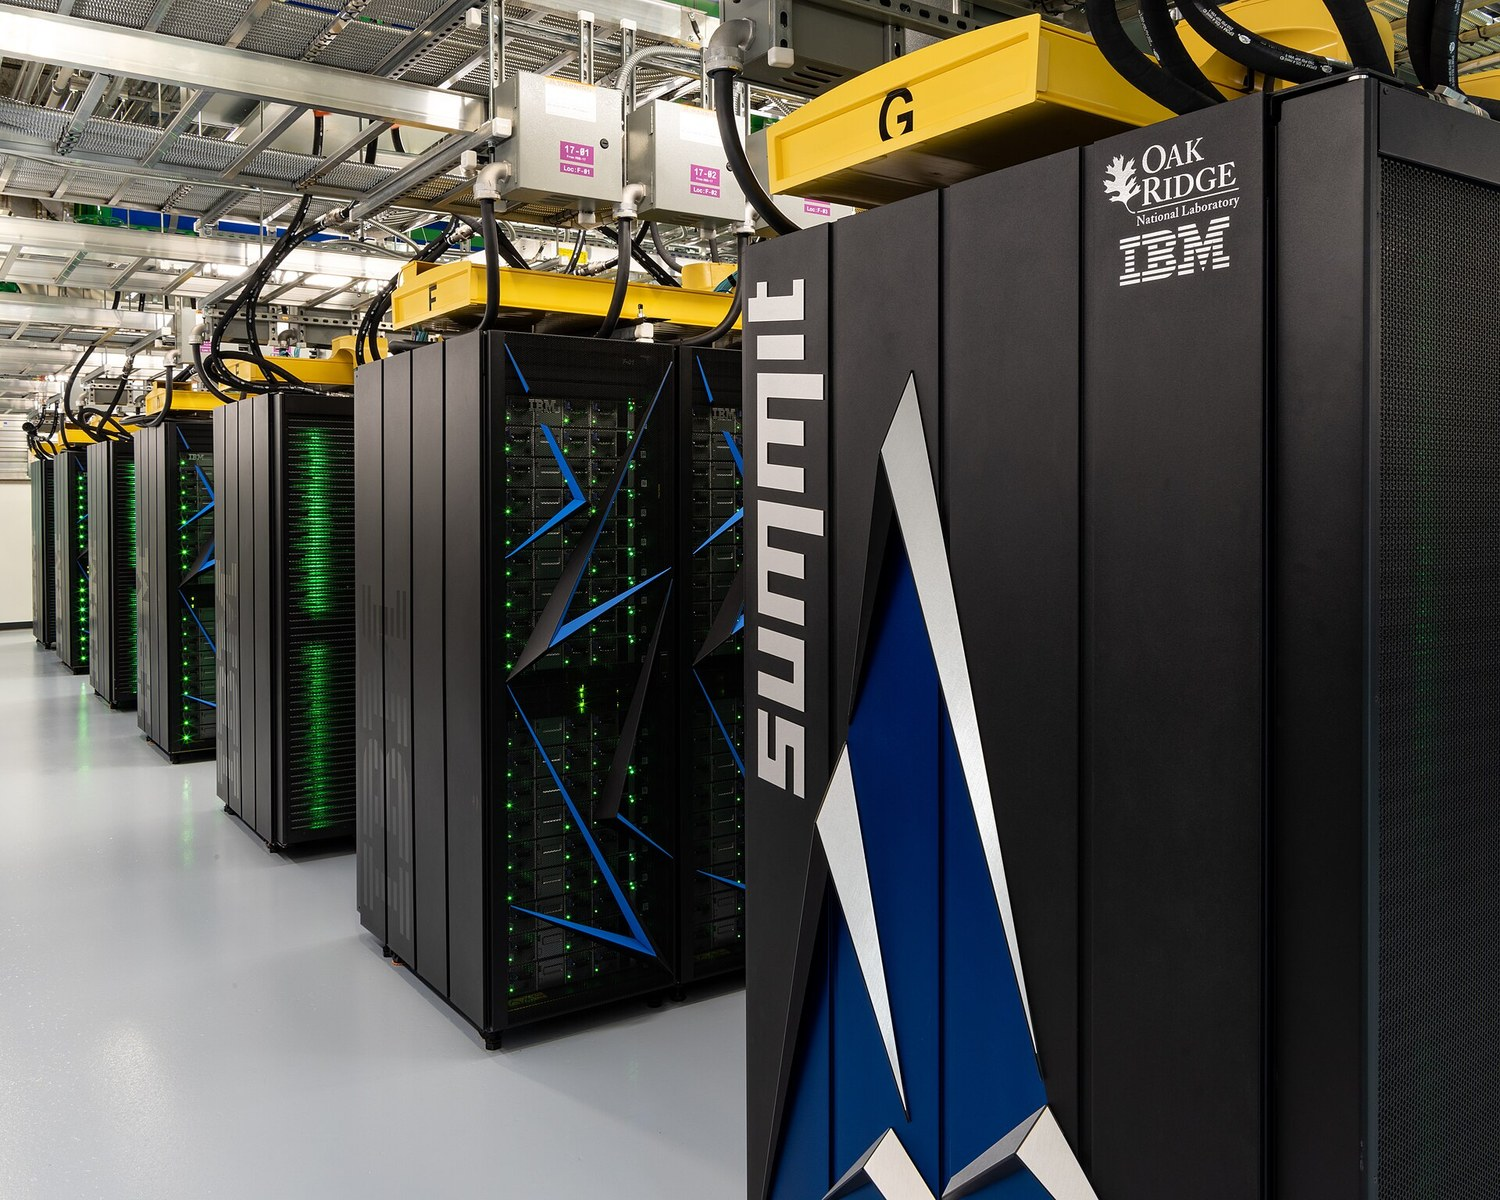
\includegraphics[width=0.72\textwidth]{../figures/summit_supercomputer.jpg}
\caption{超级计算机：粒子步总账最终要在这里付。粒子步总数乘上每步的场求解成本，就是本节的成本账；它落在真实机器上时还要除以并行效率——图上这台机器有上万块加速卡，而 PIC 的瓶颈往往不在浮点峰值，而在粒子与网格之间的数据搬运。}
\label{fig:photo-appac}
\figsource{Carlos Jones/ORNL，CC BY 2.0（Wikimedia Commons）}
\end{figure}

\section{粒子噪声：超级粒子的代价}
\label{sec:app-ac-noise}

AC.3 结尾那笔账还有一个隐形成本。用 $2\times10^{7}$ 个超级粒子代替
$8.322\times10^{22}$ 个真实粒子，省下的是算力，付出的是\textbf{噪声}。
粒子是离散地撒在相空间里的，任何一点的密度估计都带统计误差：

\begin{equation}
\frac{\delta n}{n}\approx\frac{1}{\sqrt{N_p}},
\qquad
N_p=20\;\Rightarrow\;22.361\%,
\qquad
N_p=1000\;\Rightarrow\;3.1623\%.
\label{eq:app-ac-noise}
\end{equation}

每格二十个粒子，单格相对噪声就有百分之二十二——比大多数要测量的物理效应都大。
这就是为什么 PIC 诊断量（密度剖面、温度剖面）都必须做时间平均或空间平均：

\begin{equation}
\left(\frac{\delta n}{n}\right)_{\text{平均}M\text{步}}
=\frac{1}{\sqrt{N_pM}},
\qquad
M=100\;\Rightarrow\;2.2361\%,
\label{eq:app-ac-timeavg}
\end{equation}

平均一百步把噪声降到约百分之二。反过来算：不做平均要做到 $1\%$ 精度，
每格需要 $10^{4}$ 个粒子；要 $2\%$，每格 $2500$ 个。粒子数是平方关系，
精度每提高一倍，算力涨四倍——这是 PIC 最贵的一条定律。

\begin{table}[htbp]
\centering
\small
\begin{tabular}{p{2.6cm}p{3.2cm}p{3.4cm}p{3.6cm}}
\toprule
每格粒子数 & 单格噪声 & 时间平均 $100$ 步后 & 用途 \\
\midrule
$20$ & $22.361\%$ & $2.2361\%$ & 只看定性趋势 \\
$25$ & $20\%$ & $2\%$ & 起步档 \\
$100$ & $10\%$ & $1\%$ & 看剖面形状 \\
$1000$ & $3.1623\%$ & $0.31623\%$ & 定量比较 \\
$10^{4}$ & $1\%$ & $0.1\%$ & 单步就要 $1\%$ 精度时 \\
\bottomrule
\end{tabular}
\caption{粒子噪声与粒子数的平方关系。最后一行说明「不做平均也能到 1\%」的代价。}
\label{tab:app-ac-noise}
\end{table}

\begin{tip}{噪声不是误差，是统计}{tip-app-ac-noise}
噪声没有「真值」可以对照，它本身就是有限粒子数的统计结果。
把曲线平滑一遍只会把噪声抹开，不会让它变小——要降噪声，
只能加粒子、加平均，或者改问一个对噪声不敏感的问题。
\end{tip}

{\footnotesize
\textbf{出处：}粒子噪声的 $1/\sqrt{N_p}$ 标度与时间平均降噪，
参照 Birdsall \& Langdon \emph{Plasma Physics via Computer Simulation}（1985/1991，第 3 章）
与 Tajima \emph{Computational Plasma Physics}（1989/2004，第 2 章）。
}

\section{场怎么求：泊松、FFT 与离散误差}
\label{sec:app-ac-field}

粒子把电荷放到网格上，网格再把场还给粒子。这一步的算法选择直接决定成本。
最朴素的做法是在每个格点上把所有格点的贡献加起来，运算量是 $N^2$；
用快速傅里叶变换解泊松方程，运算量降到 $N\log_2 N$：

\begin{equation}
\frac{N^2}{N\log_2 N}
=\frac{10^{12}}{1.99316\times10^{7}}=50171.7\quad(10^{6}\ \text{个格点}).
\label{eq:app-ac-fft}
\end{equation}

同一个三维问题，FFT 比直接求和快五万倍。代价是它默认周期性边界，
要换成真实边界（导体壁、开放边界）就得改用多重网格或迭代法。

快不等于准。把导数写成中心差分，本身就带来\textbf{截断误差}：

\begin{equation}
\frac{\partial^2\phi}{\partial x^2}
=\frac{\phi_{i+1}-2\phi_i+\phi_{i-1}}{\Delta x^2}+\frac{\Delta x^2}{12}\phi^{(4)},
\qquad
\frac{(\Delta x/\lambda_{De})^2}{12}=0.0833333\ (\Delta x=\lambda_{De}).
\label{eq:app-ac-trunc}
\end{equation}

取 $\Delta x=\lambda_{De}$ 时截断误差量级约百分之八。想降下来只有两条路：
缩小步长，或者提高格式阶数。二阶格式的好处是收敛快且容易验证：

\begin{equation}
\begin{aligned}
&\text{误差}\propto\Delta x^2,
\qquad
\Delta x\to\frac{\Delta x}{2}\;\Rightarrow\;\text{误差降到 }0.25\ \text{倍},\\
&\Delta x/\lambda_{De}=2/1/0.5\;\Rightarrow\;33.333\%/8.3333\%/2.0833\%.
\end{aligned}
\label{eq:app-ac-order}
\end{equation}

这张「步长减半、误差除以四」的表就是\textbf{收敛性验证}：把同一个问题在三档分辨率上各跑一遍，
如果误差不按二阶下降，说明代码里有别的东西在主导误差——往往是边界条件或诊断方法。

\begin{table}[htbp]
\centering
\small
\begin{tabular}{p{3.0cm}p{3.2cm}p{3.4cm}p{3.2cm}}
\toprule
误差来源 & 随什么变 & 本工作点的量级 & 怎么压 \\
\midrule
空间截断 & $\propto\Delta x^2$ & $8.3333\%$（$\Delta x=\lambda_{De}$） & 加密网格 / 提阶 \\
时间截断 & $\propto\Delta t^2$ & 相位 $0.00166667\ \mathrm{rad}$ 每步 & 减步长 / 高阶格式 \\
粒子统计 & $\propto1/\sqrt{N_p}$ & $22.361\%$（每格 $20$） & 加粒子 / 时间平均 \\
舍入 & 机器精度 & 约 $10^{-16}$ 相对 & 通常可忽略 \\
\bottomrule
\end{tabular}
\caption{四类误差，四种不同的「变好」方式。把它们的量级排个序，就知道该先改哪一条。}
\label{tab:app-ac-error}
\end{table}

\begin{tip}{验证与确认是两件事}{tip-app-ac-verify}
\textbf{验证}（verification）问「方程解得对不对」，靠收敛性测试和守恒量检查；
\textbf{确认}（validation）问「方程写得对不对」，靠与实验对照。
一个代码可以通过全部验证、却在确认上失败——那说明缺的不是算法，是物理。
附录 I 讲学习流程，附录 Q 讲诊断误差，本节讲的是第三种误差：算出来的误差。
\end{tip}

{\footnotesize
\textbf{出处：}FFT 泊松求解与直接求和的成本对照，参照 Press, Teukolsky, Vetterling \& Flannery
\emph{Numerical Recipes}（第 3 版，2007，第 12--13、19 章）；
PIC 中的场求解与截断误差，参照 Birdsall \& Langdon（1985/1991，第 5 章）与
Hockney \& Eastwood \emph{Computer Simulation Using Particles}（1988，第 6 章）。
}

\section{流体与 MHD：守恒格式、限制器与旋度约束}
\label{sec:app-ac-mhd}

另一半世界不用粒子，直接解流体方程。流体格式的第一原则是\textbf{守恒}：
把方程写成通量形式，让「流出这个格子的量」正好等于「流进邻居的量」，

\begin{equation}
\frac{\partial U}{\partial t}+\frac{1}{\Delta V}\oint_{\partial V}\mathbf{F}\cdot d\mathbf{A}=0
\quad\Longrightarrow\quad
\frac{d}{dt}\sum_{\text{格子}}U\Delta V
=-\sum_{\text{边界面}}\mathbf{F}\cdot\mathbf{A},
\label{eq:app-ac-flux}
\end{equation}

这样总量只会通过边界变化，不会因为离散化凭空产生或消失。
二阶精度的做法是在每个界面解一个黎曼问题，再用限制器（minmod、Van Leer 等）
把界面左右状态的斜率限住，避免在激波和间断处产生过冲。

磁场还多一条约束：$\nabla\cdot\mathbf{B}=0$ 必须\textbf{始终}成立。
离散之后它不会自动保持，误差会累积成一个假的「磁单极子」，把等离子体往错误的方向推。
两种常用解法是约束输运（constrained transport，把磁场定义在面上、用旋度更新）
与投影法（每步解一次泊松方程把散度投影掉）：

\begin{equation}
\mathbf{B}^{n+1}=\mathbf{B}^n-\Delta t\,\nabla\times\mathbf{E},
\qquad
\nabla\cdot\mathbf{B}^{n+1}=\nabla\cdot\mathbf{B}^n,
\label{eq:app-ac-divb}
\end{equation}

前者把误差压到机器精度、后者压到求解器精度，代价是每步多算一次场。

最后是内存。三维 MHD 的网格数是 PIC 的上百倍，但每个格点只存几个宏观量：

\begin{equation}
256^3\times8\ \text{个变量}\times8\ \mathrm{B}=1.07374\times10^{9}\ \mathrm{B}=1.0737\ \mathrm{GB}.
\label{eq:app-ac-memory}
\end{equation}

一 GB 内存就能装下 $256^3$ 的八个场量，这是 MHD 能跑到工程尺度的原因；
反过来，PIC 想覆盖同样的体积，粒子数会到 $10^{12}$ 以上——
两种方法不是「谁更准」，而是\textbf{谁的分辨率花在什么上}。

\begin{table}[htbp]
\centering
\small
\begin{tabular}{p{2.6cm}p{3.0cm}p{3.2cm}p{4.0cm}}
\toprule
离散方式 & 数据结构 & 优势 & 典型用途 \\
\midrule
有限差分 & 格点值 & 实现最简单 & 早期 MHD、扩散问题 \\
有限体积 & 界面通量 & 严格守恒、抓得住激波 & 现代 MHD、天体 \\
谱方法 & 傅里叶/球谐系数 & 精度指数收敛 & 湍流、周期性盒子 \\
粒子（PIC） & 宏粒子 + 网格 & 动理学、无流体假设 & 加热、尾场、快粒子 \\
\bottomrule
\end{tabular}
\caption{四类离散方式的分工。选方法的依据不是精度高低，而是「哪一层物理必须保留」。}
\label{tab:app-ac-discretization}
\end{table}

\begin{tip}{守恒律要用守恒格式写}{tip-app-ac-conservative}
同一个方程，写成守恒形式再离散，和直接离散微分形式，结果可以差很远：
后者会在激波处悄悄丢能量，而且丢多少取决于网格。
判据很简单：把总能量、总质量、总动量打印出来，看它们是不是只随边界通量变化。
\end{tip}

{\footnotesize
\textbf{出处：}通量形式与黎曼求解器参照 Godunov（1959，\emph{Matematicheskii Sbornik}
\textbf{47}, 271）与 Van Leer（1979，\emph{Journal of Computational Physics} \textbf{32}, 101）；
约束输运参照 Gardiner \& Stone（2005，\emph{Journal of Computational Physics} \textbf{205}, 509；
2008，\textbf{227}, 4123）与 Stone 等（2008，\emph{Astrophysical Journal Supplement}
\textbf{178}, 137）；隐式格式可放大步长的量级作为声明写在脚本里。
\section{估算练习}
\label{sec:app-ac-problems}
}

下面六题只用本附录的公式与工作点，把其中一个量换掉重算一遍。

\textbf{练习 1}（稀疏等离子体）：把密度降到 $1.0\times10^{19}\ \mathrm{m^{-3}}$，
温度降到 $1\ \mathrm{keV}$，磁场仍取 $5.3\ \mathrm{T}$。
求德拜长度、电子等离子体频率与德拜球内粒子数，并说明网格步长应该怎么选。

\textbf{练习 2}（网格判据）：如果偷懒取 $\Delta x=2\lambda_{De}$，
德拜屏蔽还分辨得了吗？判据要求的比值上限是多少？跑起来会看到什么现象？

\textbf{练习 3}（磁场）：把磁场降到 $2\ \mathrm{T}$，其余不变。
求电子回旋频率、允许的最大时间步长，以及这个步长下一个回旋周期有多少步。

\textbf{练习 4}（成本预算）：把模拟盒缩到 $50\lambda_{De}$，每格粒子数提到 $50$，
仍是三维、仍跑 $T_{\mathrm{end}}=1000/\omega_{pe}$。
求格点数、总粒子数、时间步数、粒子步总数与单核时间。

\textbf{练习 5}（MHD 步长）：MHD 部分把网格从 $0.01\ \mathrm{m}$ 加密到 $5\ \mathrm{mm}$，
快磁声速不变。求允许的时间步长，以及模拟 $10\tau_A$ 需要多少步。

\textbf{练习 6}（噪声预算）：每格只放 $25$ 个粒子时单格噪声是多少？
要在不做时间平均的情况下把噪声压到 $2\%$，每格需要多少粒子？
为什么「把曲线画平滑一点」不算解决办法？

\textbf{解答 1}：$\lambda_{De}=7.43394\times10^{-5}\ \mathrm{m}=74.339\ \mathrm{\mu m}$、
$\omega_{pe}=1.78399\times10^{11}\ \mathrm{rad\,s^{-1}}$、
$N_D=4.10826\times10^{6}$。
密度降十倍、温度降到九分之一，德拜长度反而变长（$\lambda_{De}\propto\sqrt{T/n}$），
所以网格可以粗一点；但德拜球内粒子数掉到四百万，只有工作点的九分之一，
\textbf{噪声会明显变大}——分辨率与信噪比是两个独立的判据。

\textbf{解答 2}：分辨不了。判据要求 $\Delta x\le\lambda_{De}$，即 $\Delta x/\lambda_{De}\le1$；
取 $2$ 意味着网格比屏蔽长度还粗，被屏蔽掉的静电场会以数值噪声的形式留在网格上，
表现为\textbf{有限网格不稳定性}：粒子被虚假的电场不断加速，动能单调上涨，
而且把 $\Delta t$ 减半也压不住。

\textbf{解答 3}：$\omega_{ce}=3.51764\times10^{11}\ \mathrm{rad\,s^{-1}}$，
$\Delta t\le0.2/\omega_{ce}=5.68563\times10^{-13}\ \mathrm{s}$，
每回旋 $31.4159$ 步。
磁场越弱、回旋越慢，允许的步长越大：$\Delta t\propto1/B$。
这也解释了为什么弱磁场装置（例如磁化惯性约束）的 PIC 模拟反而便宜。

\textbf{解答 4}：格点 $50^3=125000$，粒子数 $6.25\times10^{6}$，
步数 $8261.82$，粒子步总数 $5.16364\times10^{10}$，
单核按每秒 $10^{8}$ 粒子步算是 $516.364\ \mathrm{s}$（$0.1434\ \mathrm{h}$）。
盒缩一半、每格粒子数涨 $2.5$ 倍，成本反而只有原来（$1.65236\times10^{11}$ 粒子步）的约三分之一——
因为成本对盒尺寸是立方关系。

\textbf{解答 5}：$\Delta t=\mathrm{CFL}\cdot\Delta x/v_{ms}
=3.39699\times10^{-10}\ \mathrm{s}$，模拟 $10\tau_A$ 需要 $24962.9$ 步。
网格减半、步长减半、步数加倍：显式格式的总成本按 $\Delta x^{-4}$ 涨（三维），
这是隐式格式存在的理由。

\textbf{解答 6}：单格噪声 $20\%$；要 $2\%$ 需要每格 $2500$ 个粒子。
平滑只是把噪声在空间上抹开，噪声的\textbf{统计涨落幅度}并没有变小，
相邻点之间的关联反而被做出来了——那等于伪造了信息。
正确做法只有三条：加粒子、做时间平均、或者换一个对噪声不敏感的诊断量。

\section{来源、分级与版权说明}
\label{sec:app-ac-source}

\begingroup\small
本附录的数字分三级，和前面各附录同一口径。

工作点与附录 M 到 AB 完全一致：$n_e=1.0\times10^{20}\ \mathrm{m^{-3}}$、
$T_e=9.194\ \mathrm{keV}$、$B=5.3\ \mathrm{T}$、$Z_{\mathrm{eff}}=2$、$m_i=2.5m_p$；
模拟盒取 $100\lambda_{De}$、$\Delta x=\lambda_{De}$、每格 $20$ 个粒子、
$T_{\mathrm{end}}=1000/\omega_{pe}$、$\Delta t=0.2/\omega_{ce}$；
MHD 部分取 $\Delta x=0.01\ \mathrm{m}$、$256^3$ 网格、$\mathrm{CFL}=0.5$。

\textbf{声明级}：库仑对数 $\ln\Lambda=17$、单核每秒 $10^{8}$ 粒子步、
GPU 每秒 $10^{9}$ 粒子步、每个格点 $8$ 个变量 $\times8\ \mathrm{B}$、
隐式格式允许把步长放大 $100$ 倍量级——这些是\textbf{量级假设}，
写在脚本开头的 \texttt{[DECLARED]} 段里，正文引用时会说明是声明值。

\textbf{文献级}：推进器、CFL 条件、限制器、约束输运这些\textbf{方法}的出处，
只给书名、作者、年份与卷期页。本附录
因此不给链接、不给页码区间。

\begin{table}[htbp]
\centering
\small
\begin{tabular}{p{3.4cm}p{4.0cm}p{4.6cm}}
\toprule
来源 & 借用的内容 & 本附录的处理 \\
\midrule
Birdsall \& Langdon（1985/1991） & PIC 分辨率判据、噪声标度、Boris 步 & 只借结论与公式形式；数值全部按本工作点重算 \\
Hockney \& Eastwood（1988） & 场求解与截断误差 & 只借误差阶数的结论 \\
Tajima（1989/2004） & 成本估算、超级粒子 & 只借用词与量级框架 \\
Press 等（2007） & FFT 解泊松的运算量 & 只借 $N\log_2N$ 这一形式，数值自算 \\
Boris（1970）、Vay（2008） & 推进器构造 & 只借旋转形式与守恒性质 \\
Courant 等（1928） & CFL 条件 & 只借用判据形式 \\
Godunov（1959）、Van Leer（1979） & 通量形式与限制器 & 只借方法名与适用场合 \\
Gardiner \& Stone（2005/2008）、Stone 等（2008） & 约束输运 & 只借 $\nabla\cdot\mathbf{B}$ 的处理思路 \\
\bottomrule
\end{tabular}
\caption{本附录的借鉴来源与处理边界。全部为方法层面的引用，不含任何原文文字、表格或数值。}
\label{tab:app-ac-source}
\end{table}

关于版权，本附录明确声明：

一、\textbf{不复制}任何原书的文字表述、章节编号、插图与习题；正文全部自拟，
例题与练习的题材取自公共的方法学常识，数值全部独立复算。

二、\textbf{不复制}任何软件的手册文本与代码片段；正文只描述算法结构，
不给可直接运行的实现（附录 G 已给出上手路线，其代码由本教材自行编写）。

三、\textbf{不复制}任何文献中的性能基准数字（例如某代码在某 GPU 上的加速比）：
这类数随硬件变化极快，只用本教材自己的量级估算。

四、\textbf{不复制}任何未经验证的参数推荐值（例如「每格 100 个粒子最好」）：
只给判据与代价曲线，把选择权留给读者自己的工作点。

\begin{tip}{学会说「这不算」}{tip-app-ac-honest}
数值工作的诚实体现在三句话上：这个数是我算的，那个数是我假设的，
还有一个数是别人测的。混在一起讲，结论就没法被检验——
本附录的每一个数字，都能在 \texttt{tools/\allowbreak{}calc/\allowbreak{}appAC\_calc.py} 的输出里找到出处。
\end{tip}

\textbf{出处：}本节的来源分级与版权口径，沿用本教材附录 E（分级自学书单）与
附录 I（学习策略）的既定做法；方法层面的引用见上表，
对应的文献信息与 AC.1--AC.6 各节的「出处：」段一致。
\endgroup
